\documentclass[tikz,border=8pt]{standalone}
\usepackage{amsmath,amssymb}
\usetikzlibrary{arrows.meta,automata,positioning,quotes}
\begin{document}
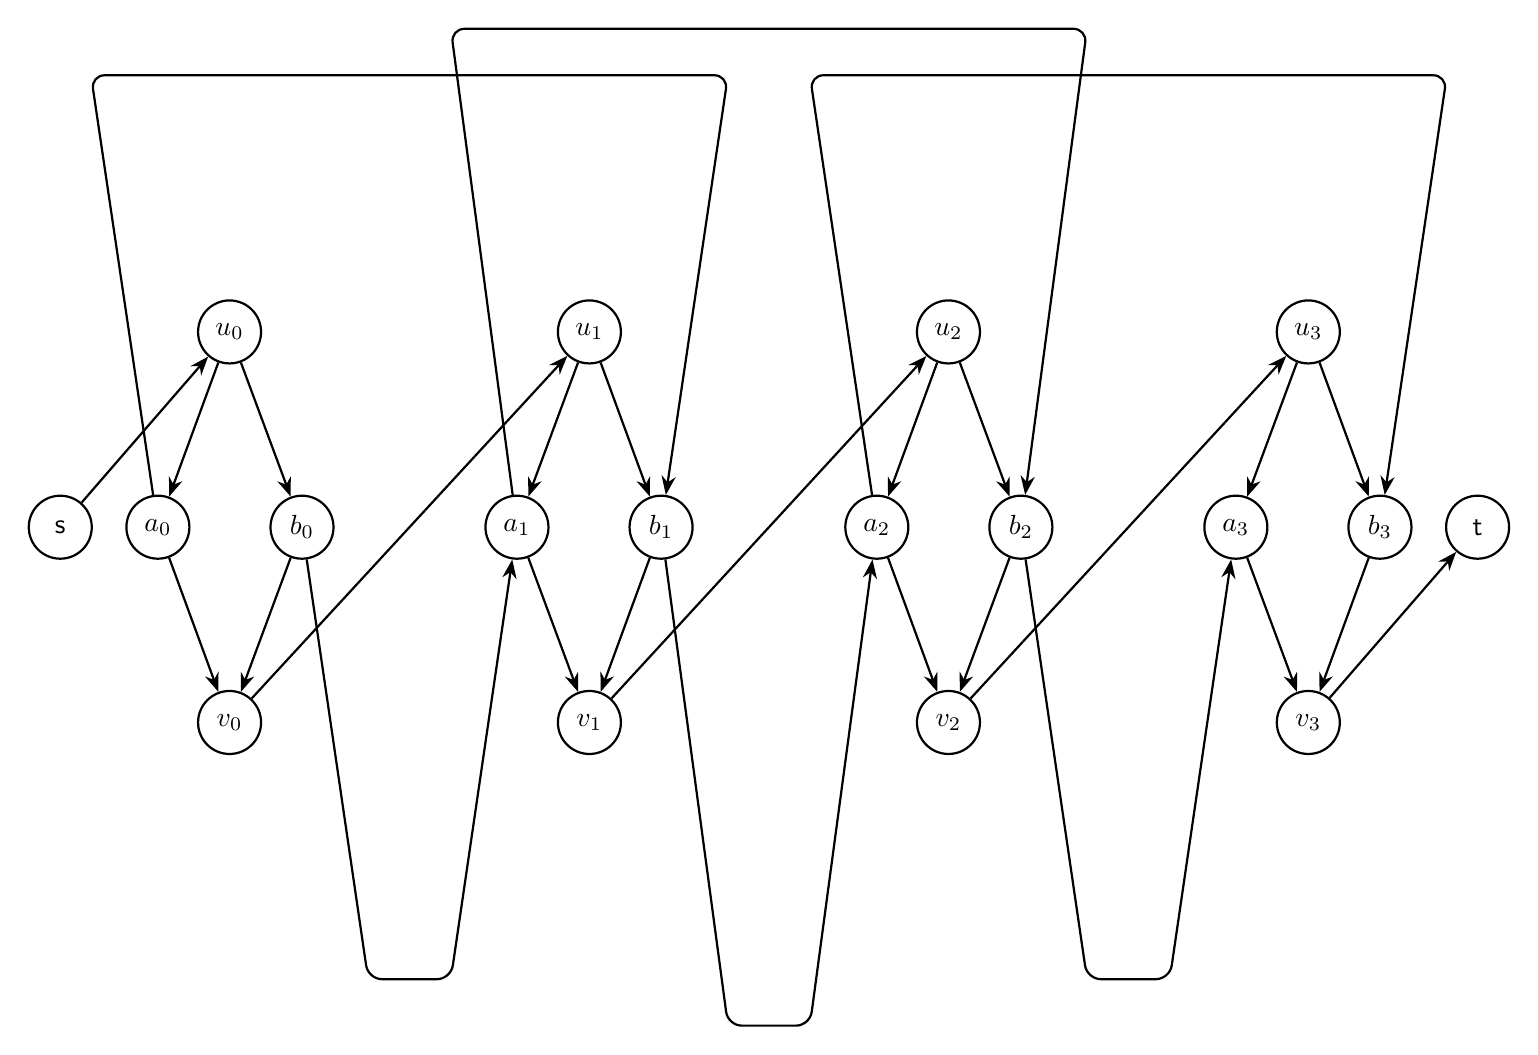
\begin{tikzpicture}[x=1cm,y=1cm]
\tikzset{
  graphnode/.style={circle,draw,thick,minimum size=8mm,inner sep=1pt,font=\sffamily},
  directed/.style={-{Stealth[length=2.4mm]},thick},
  undirected/.style={thick}
}
\node[graphnode] (n_s) at (-9.00,0.00) {s};
\node[graphnode] (n_t) at (9.00,0.00) {t};
\node[graphnode] (n_u_0) at (-6.85,2.48) {$u_{0}$};
\node[graphnode] (n_v_0) at (-6.85,-2.48) {$v_{0}$};
\node[graphnode] (n_a_0) at (-7.76,0.00) {$a_{0}$};
\node[graphnode] (n_b_0) at (-5.93,0.00) {$b_{0}$};
\node[graphnode] (n_u_1) at (-2.28,2.48) {$u_{1}$};
\node[graphnode] (n_v_1) at (-2.28,-2.48) {$v_{1}$};
\node[graphnode] (n_a_1) at (-3.20,0.00) {$a_{1}$};
\node[graphnode] (n_b_1) at (-1.37,0.00) {$b_{1}$};
\node[graphnode] (n_u_2) at (2.28,2.48) {$u_{2}$};
\node[graphnode] (n_v_2) at (2.28,-2.48) {$v_{2}$};
\node[graphnode] (n_a_2) at (1.37,0.00) {$a_{2}$};
\node[graphnode] (n_b_2) at (3.20,0.00) {$b_{2}$};
\node[graphnode] (n_u_3) at (6.85,2.48) {$u_{3}$};
\node[graphnode] (n_v_3) at (6.85,-2.48) {$v_{3}$};
\node[graphnode] (n_a_3) at (5.93,0.00) {$a_{3}$};
\node[graphnode] (n_b_3) at (7.76,0.00) {$b_{3}$};
\draw[directed] (n_u_0) -- (n_a_0);
\draw[directed] (n_u_0) -- (n_b_0);
\draw[directed] (n_a_0) -- (n_v_0);
\draw[directed] (n_b_0) -- (n_v_0);
\draw[directed] (n_u_1) -- (n_a_1);
\draw[directed] (n_u_1) -- (n_b_1);
\draw[directed] (n_a_1) -- (n_v_1);
\draw[directed] (n_b_1) -- (n_v_1);
\draw[directed] (n_u_2) -- (n_a_2);
\draw[directed] (n_u_2) -- (n_b_2);
\draw[directed] (n_a_2) -- (n_v_2);
\draw[directed] (n_b_2) -- (n_v_2);
\draw[directed] (n_u_3) -- (n_a_3);
\draw[directed] (n_u_3) -- (n_b_3);
\draw[directed] (n_a_3) -- (n_v_3);
\draw[directed] (n_b_3) -- (n_v_3);
\draw[directed] (n_s) -- (n_u_0);
\draw[directed] (n_v_0) -- (n_u_1);
\draw[directed] (n_v_1) -- (n_u_2);
\draw[directed] (n_v_2) -- (n_u_3);
\draw[directed] (n_v_3) -- (n_t);
\draw[directed,rounded corners=5pt] (n_a_0) -- (-8.61,5.74) -- (-0.52,5.74) -- (n_b_1);
\draw[directed,rounded corners=5pt] (n_b_0) -- (-5.09,-5.74) -- (-4.04,-5.74) -- (n_a_1);
\draw[directed,rounded corners=5pt] (n_a_1) -- (-4.04,6.33) -- (4.04,6.33) -- (n_b_2);
\draw[directed,rounded corners=5pt] (n_b_1) -- (-0.52,-6.33) -- (0.52,-6.33) -- (n_a_2);
\draw[directed,rounded corners=5pt] (n_a_2) -- (0.52,5.74) -- (8.61,5.74) -- (n_b_3);
\draw[directed,rounded corners=5pt] (n_b_2) -- (4.04,-5.74) -- (5.09,-5.74) -- (n_a_3);
\end{tikzpicture}
\end{document}
